% 4_results_and_discussion.tex
\section{Resultados y Discusión}
\subsection{Cometa Halley}
Como se observa en la Figura \ref{fig:halley_orbit}, en ausencia de otros cuerpos, la trayectoria del cometa Halley describe una cónica cerrada fuertemente elongada alrededor del Sol. De acuerdo con la simulación, en la que se empleo un $\Delta t = 0.001$ años y tiempo total de 228 años, se obtuvo que su distancia máxima al Sol (afelio) es de $r_{\max} = 35.3458 \, \text{AU}$. La velocidad orbital alcanza un máximo absoluto de $v_{\max} = 11.4728 \, \text{AU/año}$. Relativo a la arquitectura del Sistema Solar exterior, el afelio de Halley no supera el afelio de Plutón, pero sí es mayor que el perihelio de este último, alcanzando aproximadamente un $89.5\%$ de la distancia orbital media del planeta enano.
    

\begin{figure}[htbp]
    \centering
    \href{https://youtu.be/lc274xHxq8g}{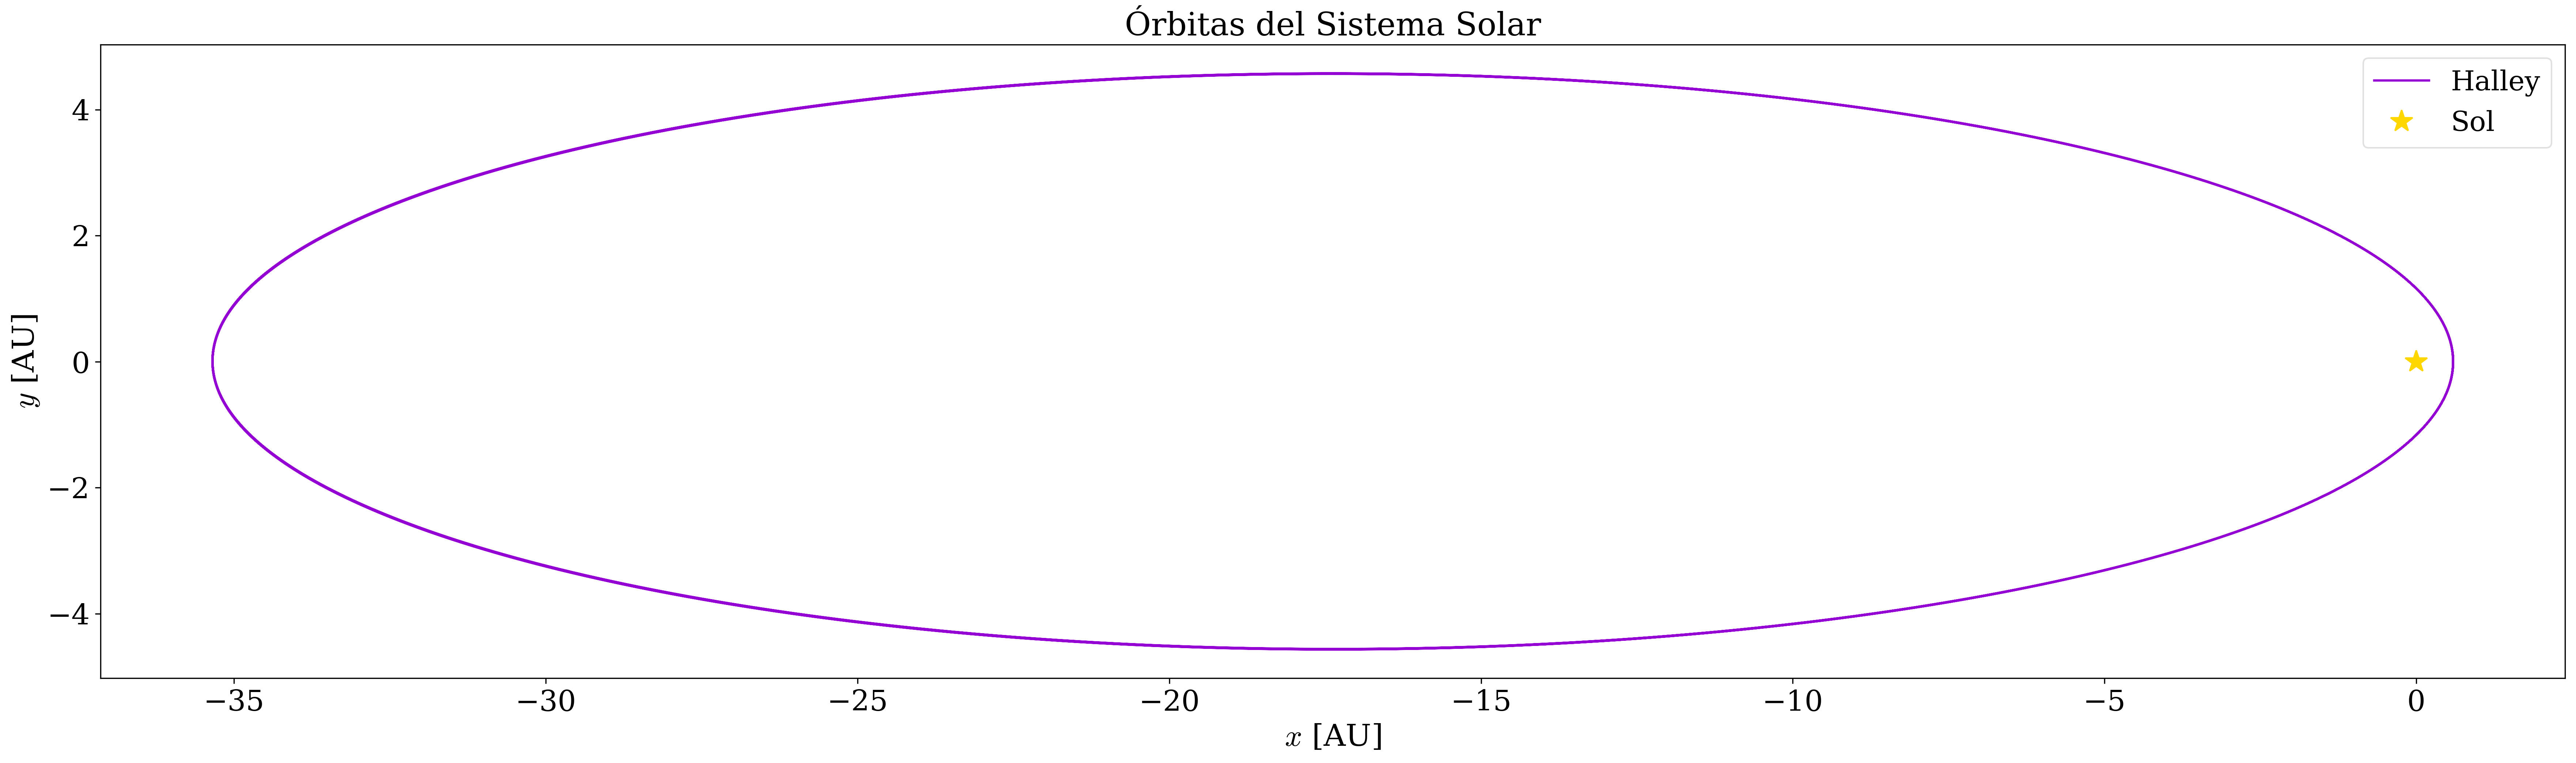
\includegraphics[width=\textwidth]{figures_tex/halley_sun.png}}
    \caption{Trayectoria orbital 2D del Cometa Halley (púrpura) en el plano orbital, con el Sol (estrella amarilla) ubicado en uno de los focos de la elipse.}
    \label{fig:halley_orbit}
\end{figure}


La integración numérica del sistema preserva de manera robusta los invariantes físicos fundamentales a lo largo del tiempo de simulación, tal y como se aprecia en la Figura \ref{fig:energy_momentum}. Los picos recurrentes en $K$ y $U$ son indicativos de los pasos por el perihelio, donde la velocidad orbital y la profundidad en el pozo gravitatorio se maximizan. La magnitud de la variación del momento angular ($\Delta L \sim 10^{-13}$) evidencia que las fluctuaciones están dominadas exclusivamente por la precisión de punto flotante relativo) propia de la arquitectura computacional. Esto confirma la naturaleza simpléctica del método de Velocity Verlet.

\begin{figure}[htbp]
    \centering
    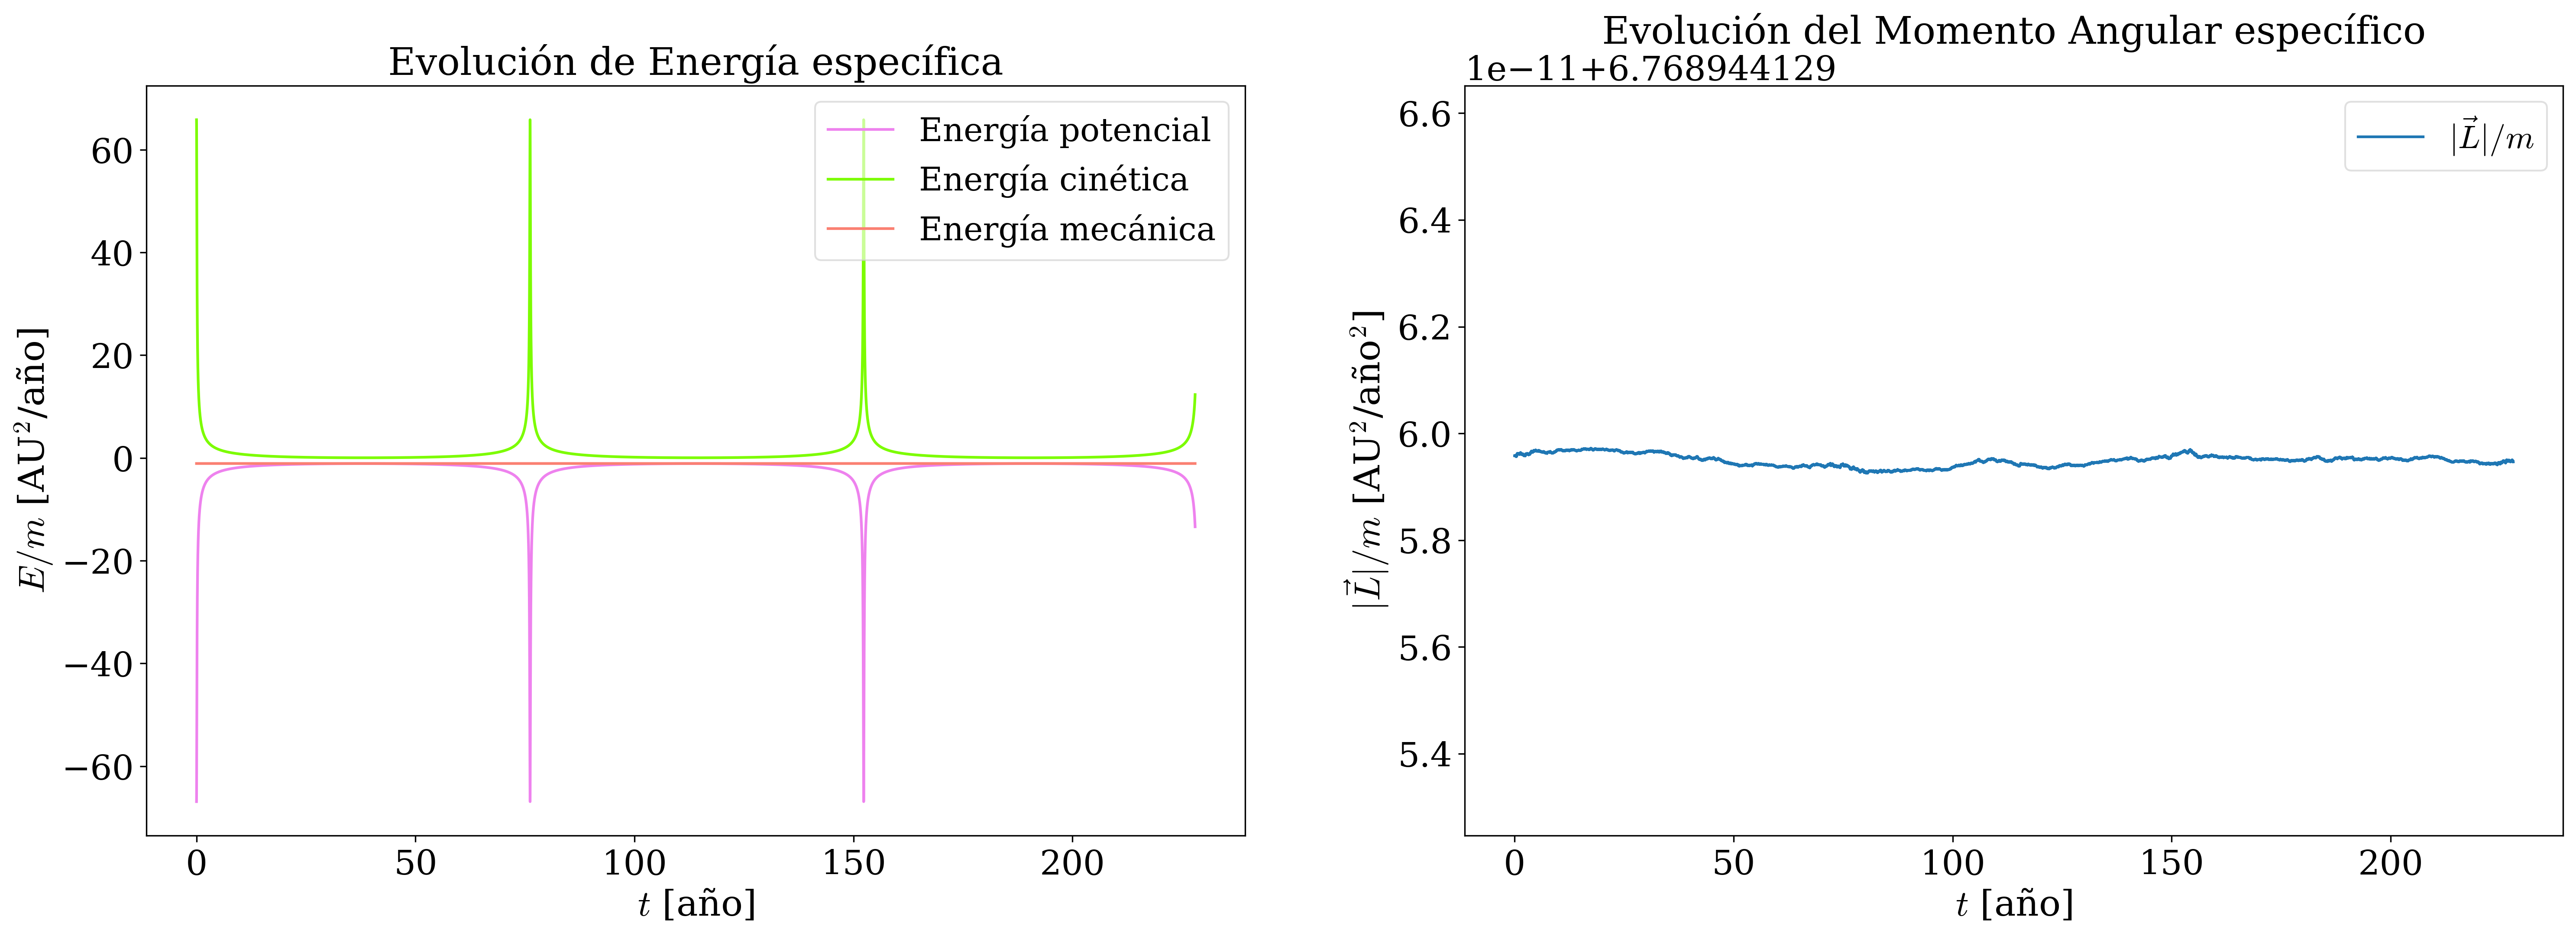
\includegraphics[width=1\textwidth]{figures_tex/energy_momentum.png}
    \caption{Evolución temporal de las energías cinética, potencial y mecánica (izquierda) y magnitud del momento angular (derecha) por unidad de masa.}
    \label{fig:energy_momentum}
\end{figure}




Para determinar la precesión del perihelio ($\dot{\omega}$) del cometa Halley bajo la perturbación de Júpiter, se analizó la respuesta del sistema escalando paramétricamente la masa joviana ($M_J$). Las Figuras \ref{fig:why_extrapolation} y \ref{fig:extrapolation} muestran que, para masas inferiores a $5M_J$, la señal de precesión es indeterminada o no confiable. En consecuencia, se realizó una extrapolación lineal a partir del intervalo $[5M_J, 11.5M_J]$ hacia el valor real de la masa ($1M_J$). El resultado obtenido para la tasa de precesión, empleando $\Delta t = 0.005$ años, es:$$\dot{\omega} = -1.57 \times 10^{-4} \text{ rad/año}$$ 
El signo negativo indica precesión en sentido horario.

\begin{figure}[htbp]
    \centering
    \begin{minipage}{0.48\textwidth}
        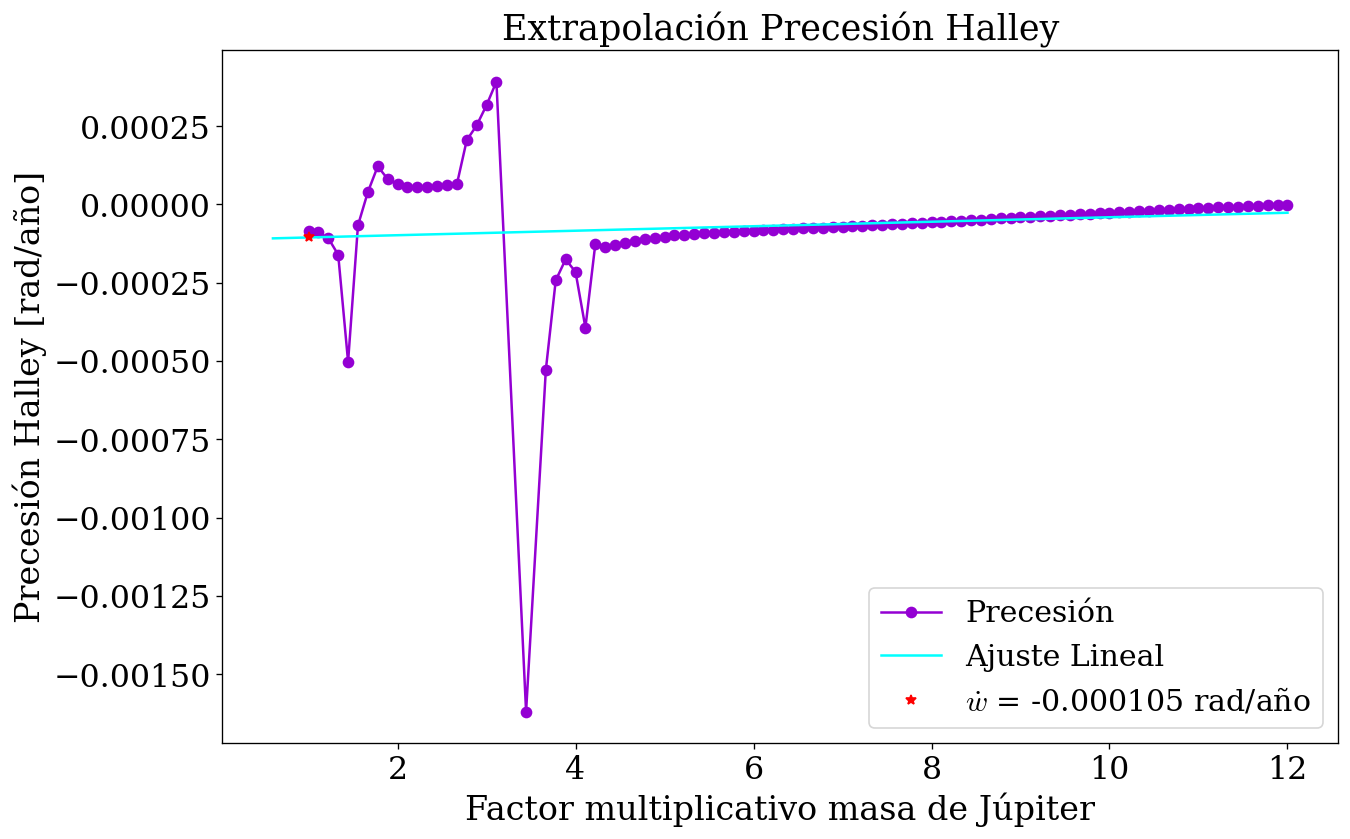
\includegraphics[width=\textwidth]{figures_tex/why_extrapolation.png}
        \caption{Variación de la tasa de precesión para factores de masa de Júpiter en el intervalo $[1, 12]$ y su ajuste lineal.}
        \label{fig:why_extrapolation}
    \end{minipage}\hfill
    \begin{minipage}{0.48\textwidth}
        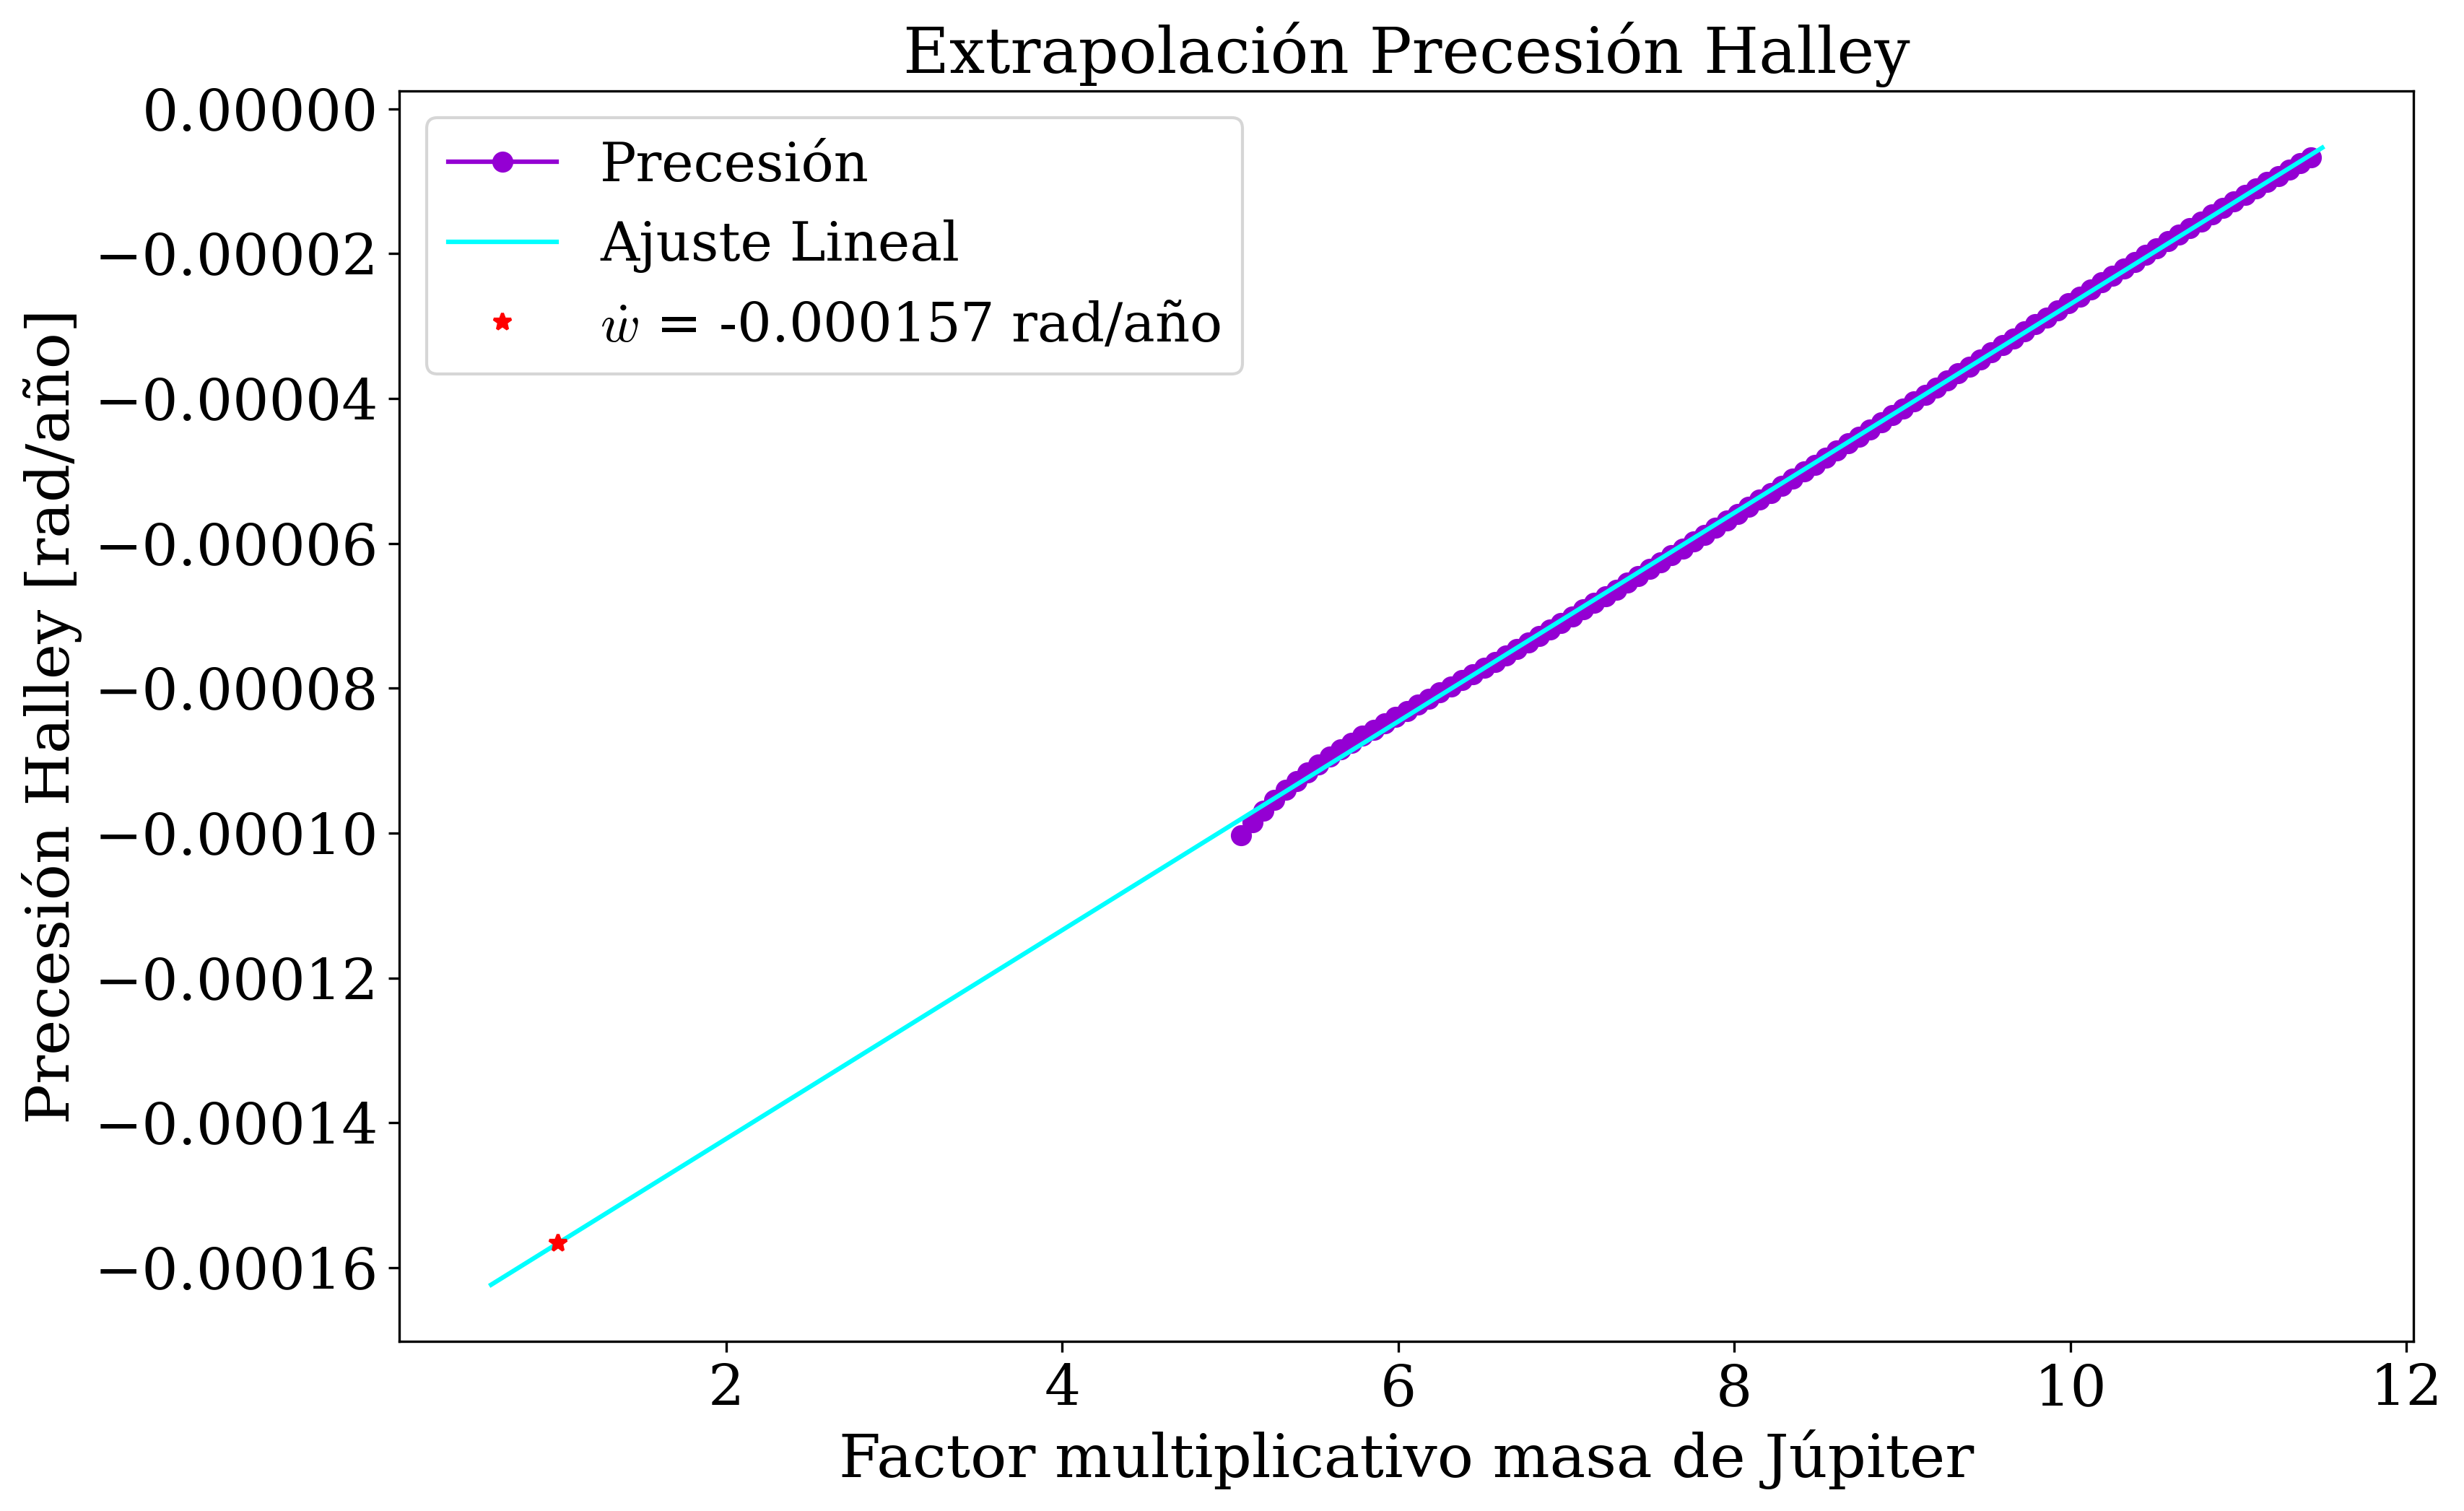
\includegraphics[width=\textwidth]{figures_tex/extrapolation.png}
        \caption{Variación de la tasa de precesión para factores de masa de Júpiter en la región sin fluctuaciones ($[5, 11.5]$) y su ajuste lineal.}
        \label{fig:extrapolation}
    \end{minipage}
\end{figure}



\subsection{Puntos de Lagrange}
El análisis del entorno dinámico Tierra-Luna se visualiza mediante la superficie del pseudopotencial en el Problema Circular Restringido de los Tres Cuerpos (PCR3C), mostrado en la Figura \ref{fig:potencial_eff}.

\begin{figure}[H]
    \centering
    \begin{minipage}{0.48\textwidth}
        \centering
        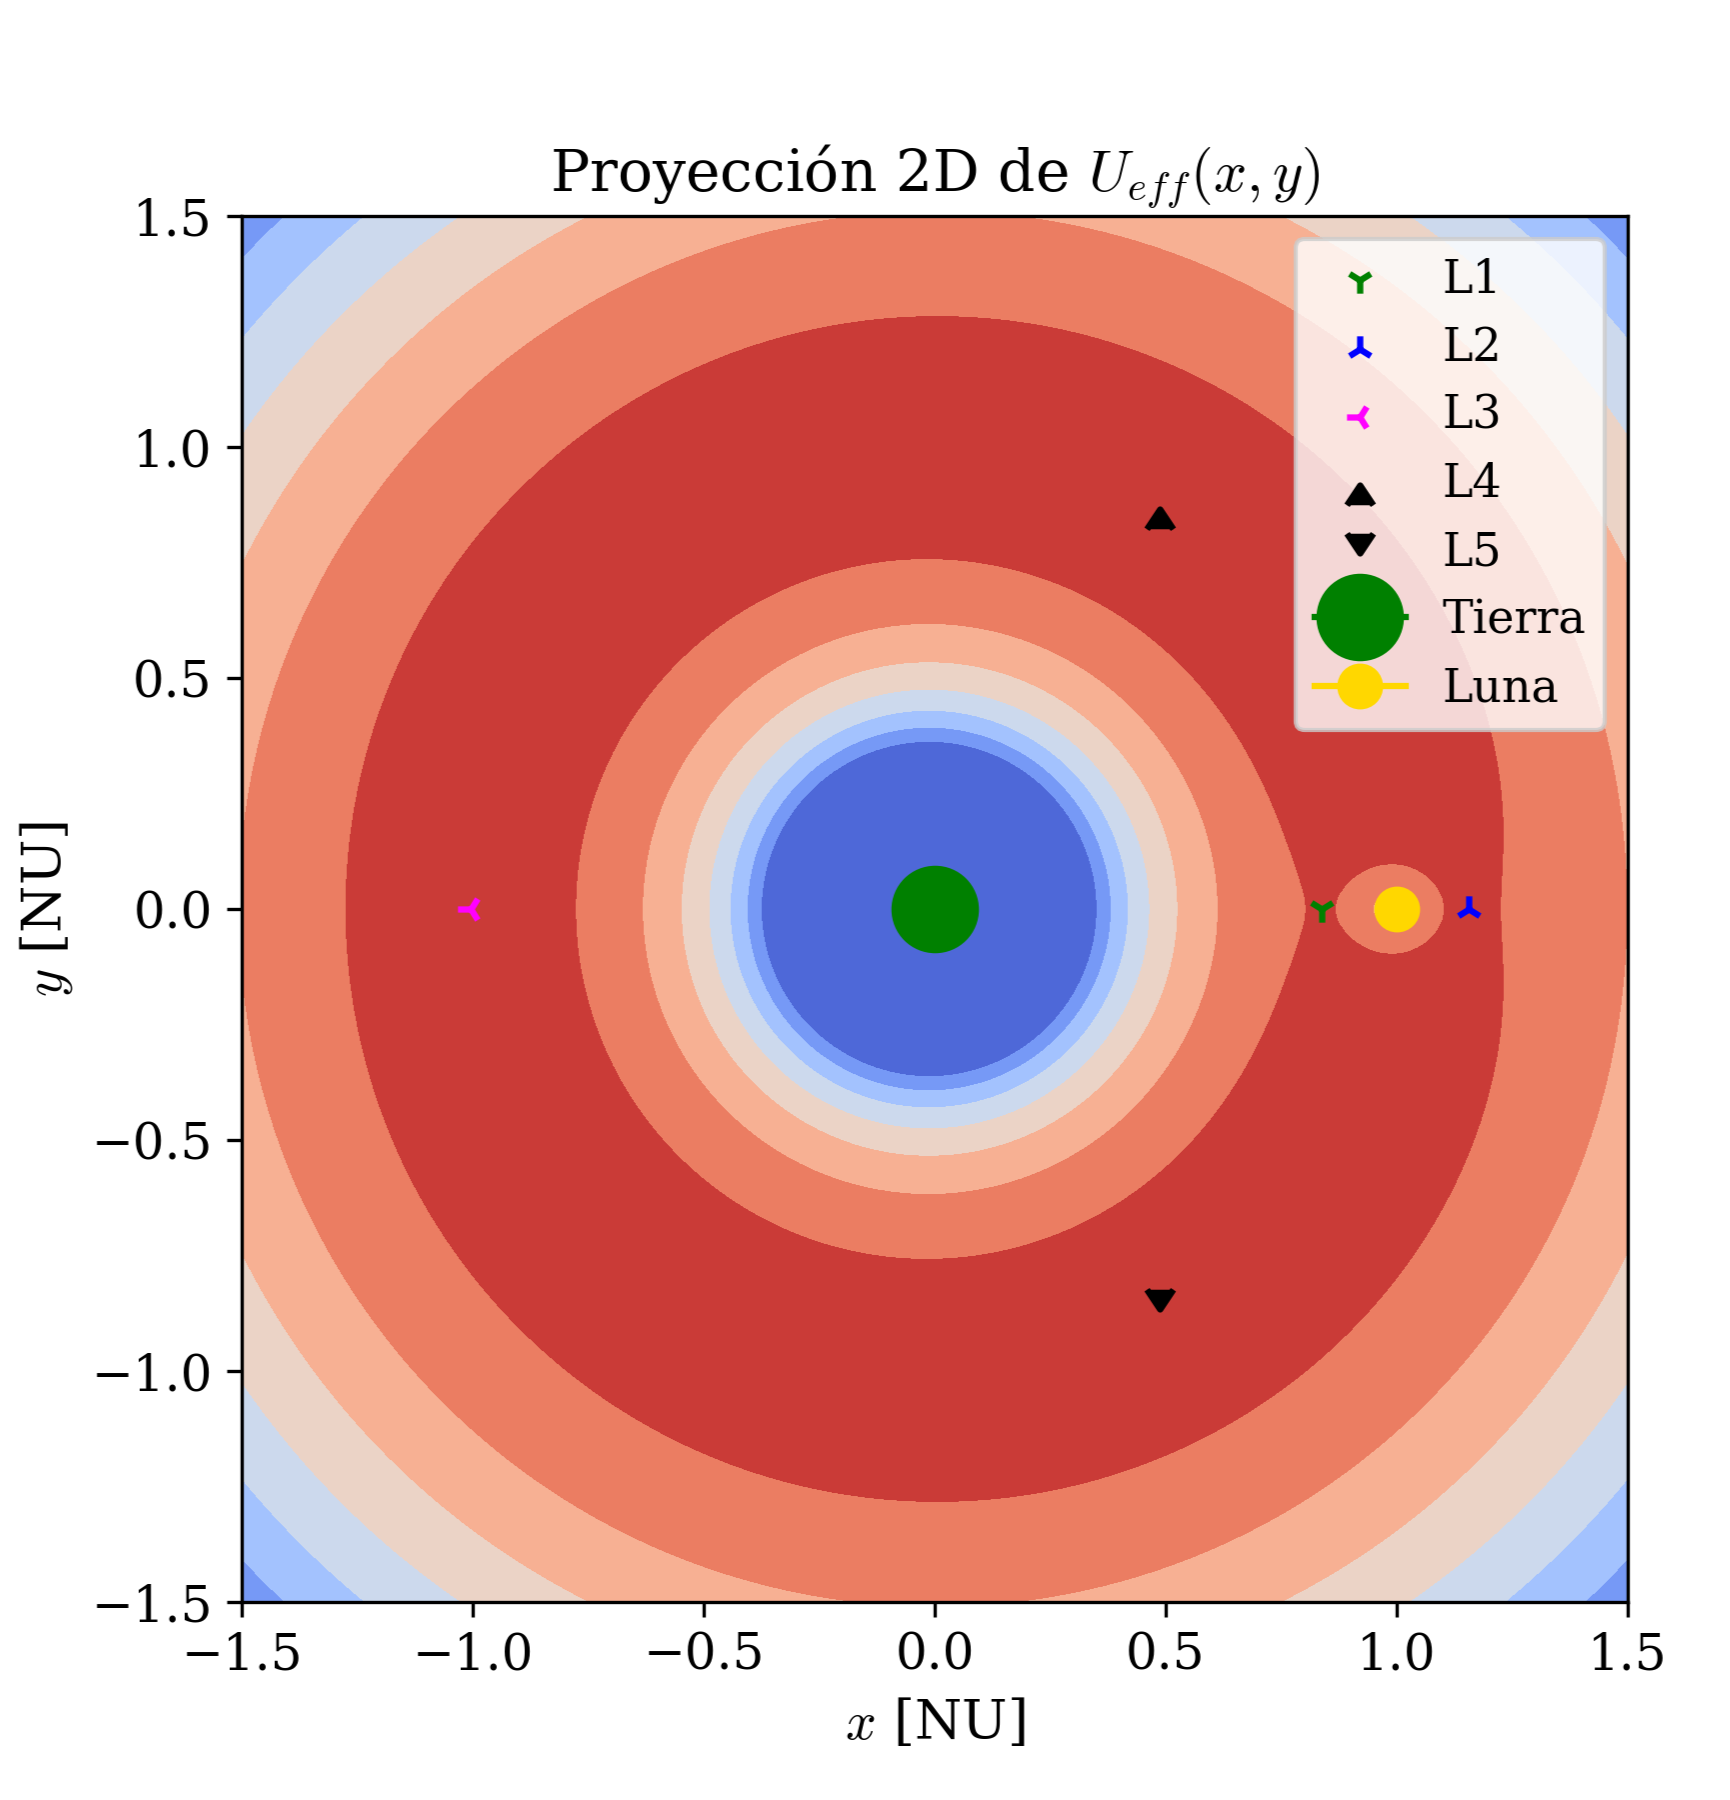
\includegraphics[width=\textwidth]{figures_tex/potencial_2d.png}
    \end{minipage}\hfill
    \begin{minipage}{0.48\textwidth}
        \centering
        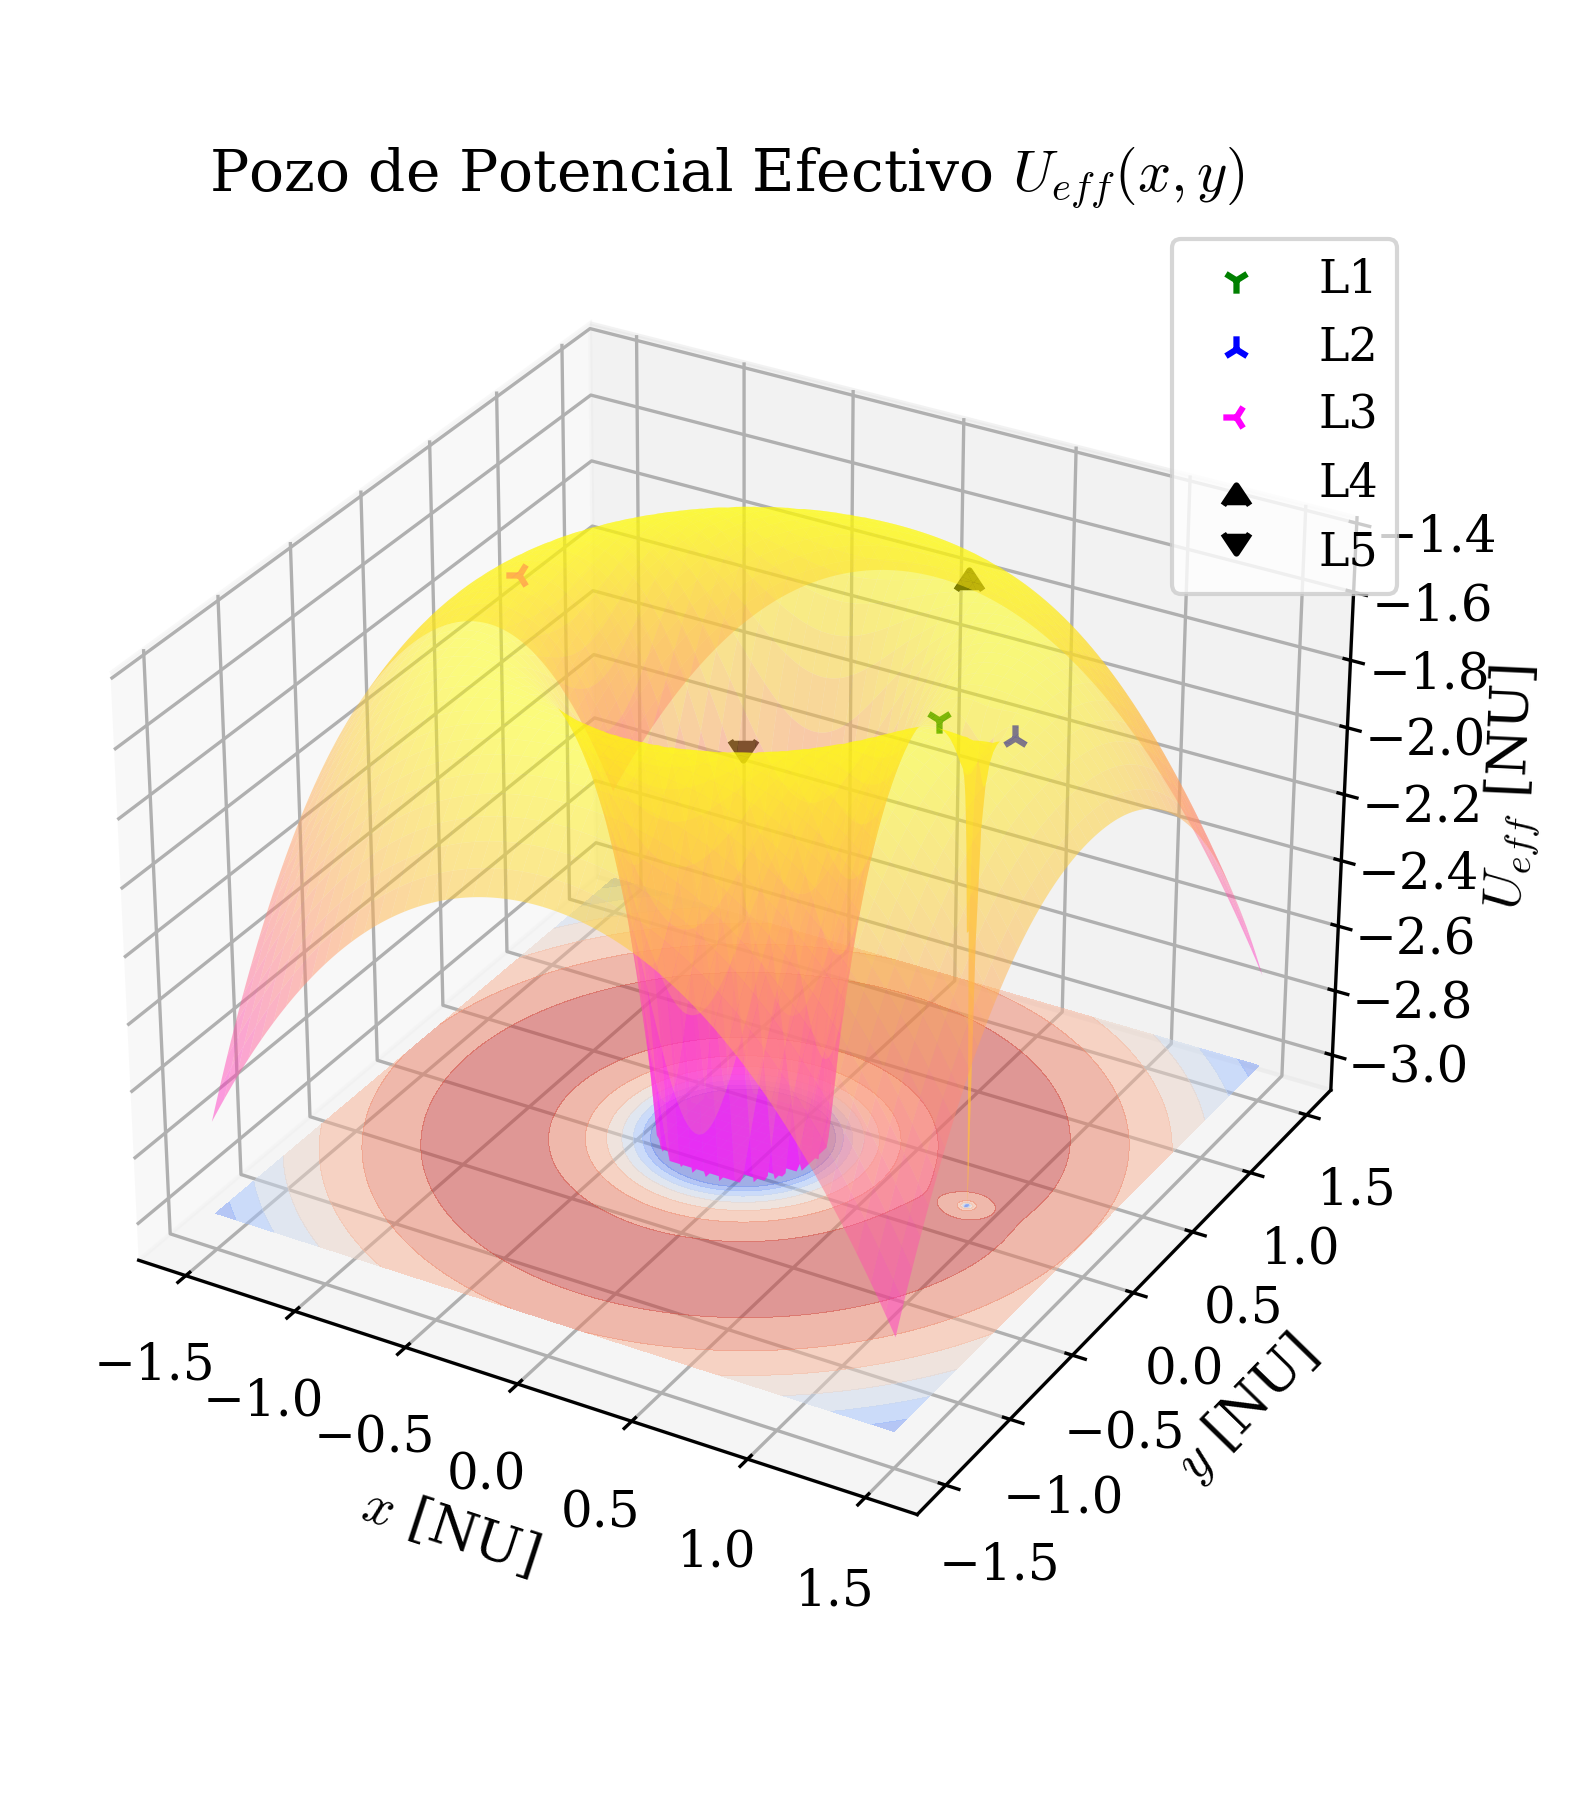
\includegraphics[width=\textwidth]{figures_tex/potencial_3d.png}
    \end{minipage}
    \caption{Proyección en 2D con curvas de nivel (izquierda) y superficie 3D (derecha) del pozo de potencial efectivo $U_{\text{eff}}(x,y)$ en el sistema Tierra-Luna, mostrando la ubicación de los cinco puntos de Lagrange.}
    \label{fig:potencial_eff}
\end{figure}










La topología del potencial incorpora tanto las atracciones gravitatorias newtonianas ($\propto -1/r$) como el término centrífugo del sistema rotante ($\propto -r^2$). Visualmente, la métrica revela que $L_1, L_2$ y $L_3$ son puntos de silla topológicos (mínimos en una dirección, máximos en la ortogonal). Curiosamente, $L_4$ y $L_5$ representan máximos locales del potencial efectivo, lo que intuitivamente sugeriría inestabilidad estática, haciendo necesaria la evaluación de fuerzas dependientes de la velocidad.

% ---------------------------------------------------------
% BLOQUE 3: Estabilidad de los Puntos de Lagrange
% ---------------------------------------------------------
Para verificar la estabilidad dinámica predicha, la Figura \ref{fig:lagrange_orbits} ilustra la evolución temporal de pequeñas perturbaciones ($\delta_1$, puramente espacial; $\delta_2$, espacial y cinemática) aplicadas sobre las posiciones de equilibrio exactas para los puntos $L1-L4$, omitiendo el punto $L_5$ por su simetría especular respecto al eje Tierra-Luna con $L_4$.

\begin{figure}[htbp]
    \centering
    \begin{minipage}{0.48\textwidth}
    \href{https://www.youtube.com/watch/RlNEgH9QZA4?feature=share}{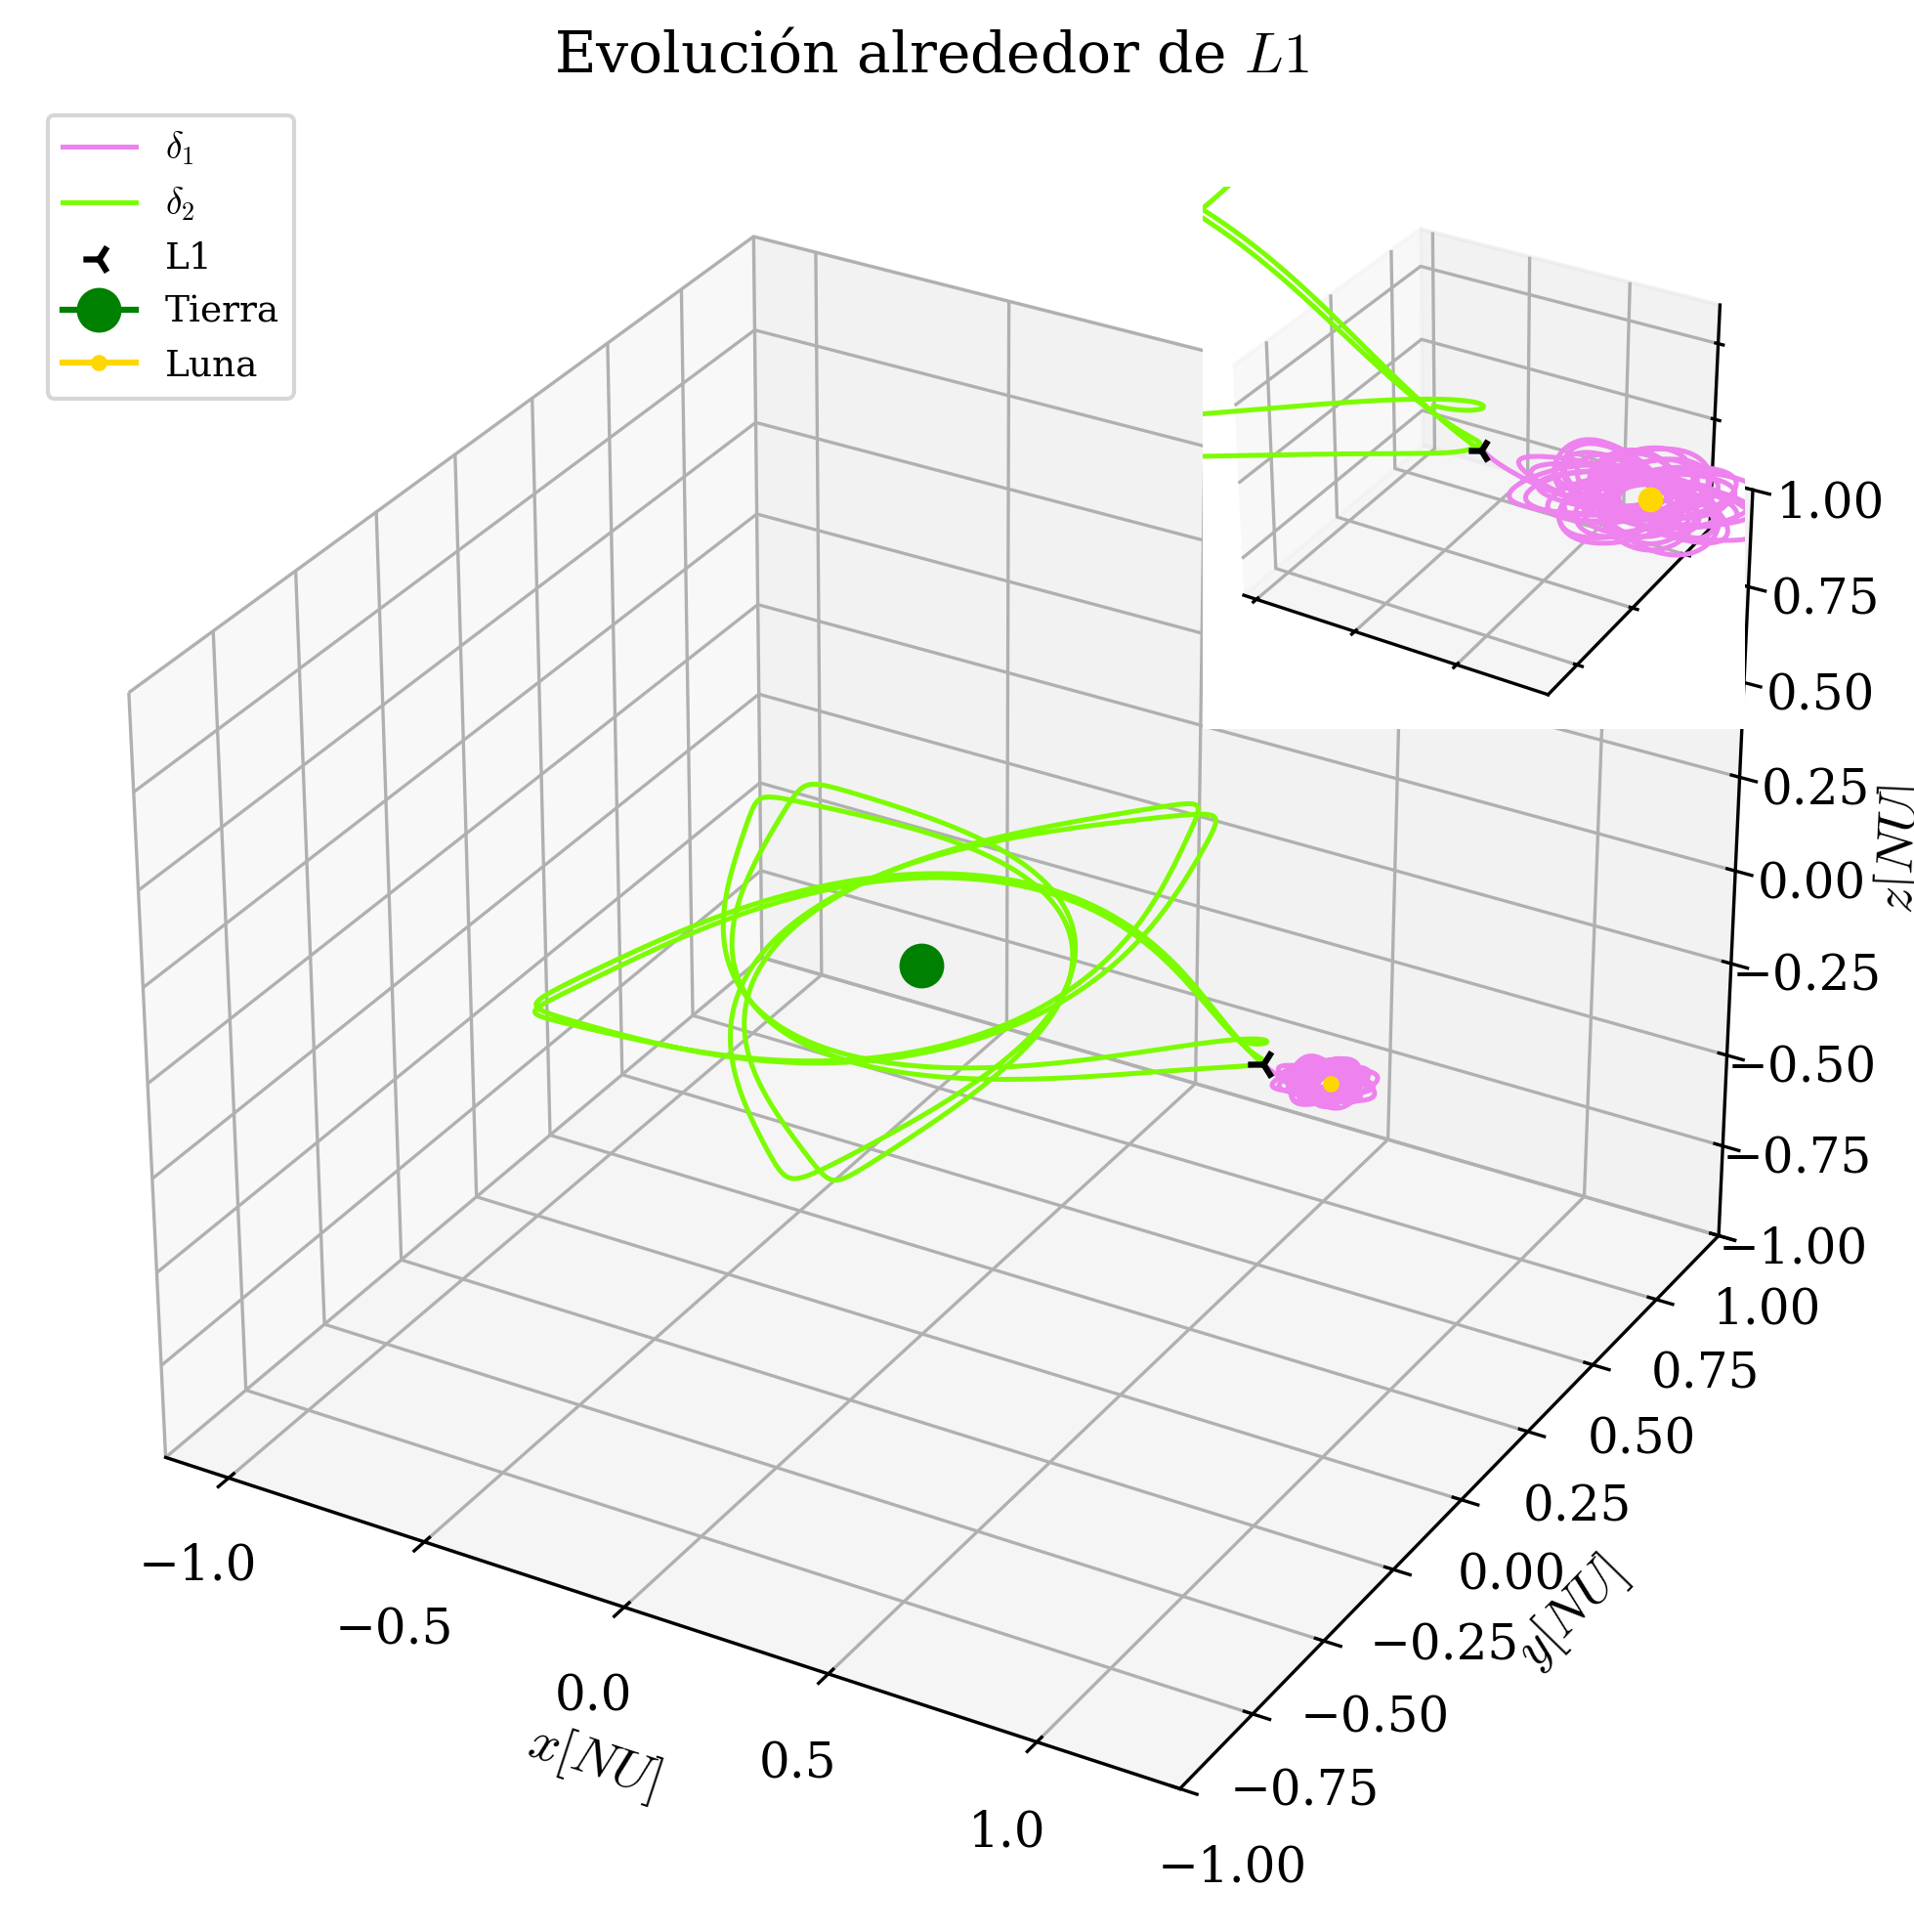
\includegraphics[width=\textwidth]{figures_tex/orbit_lagrange_L1.png}}
    \end{minipage}
    \begin{minipage}{0.48\textwidth}
        \href{https://www.youtube.com/watch?v=51BHZS_yqqw}{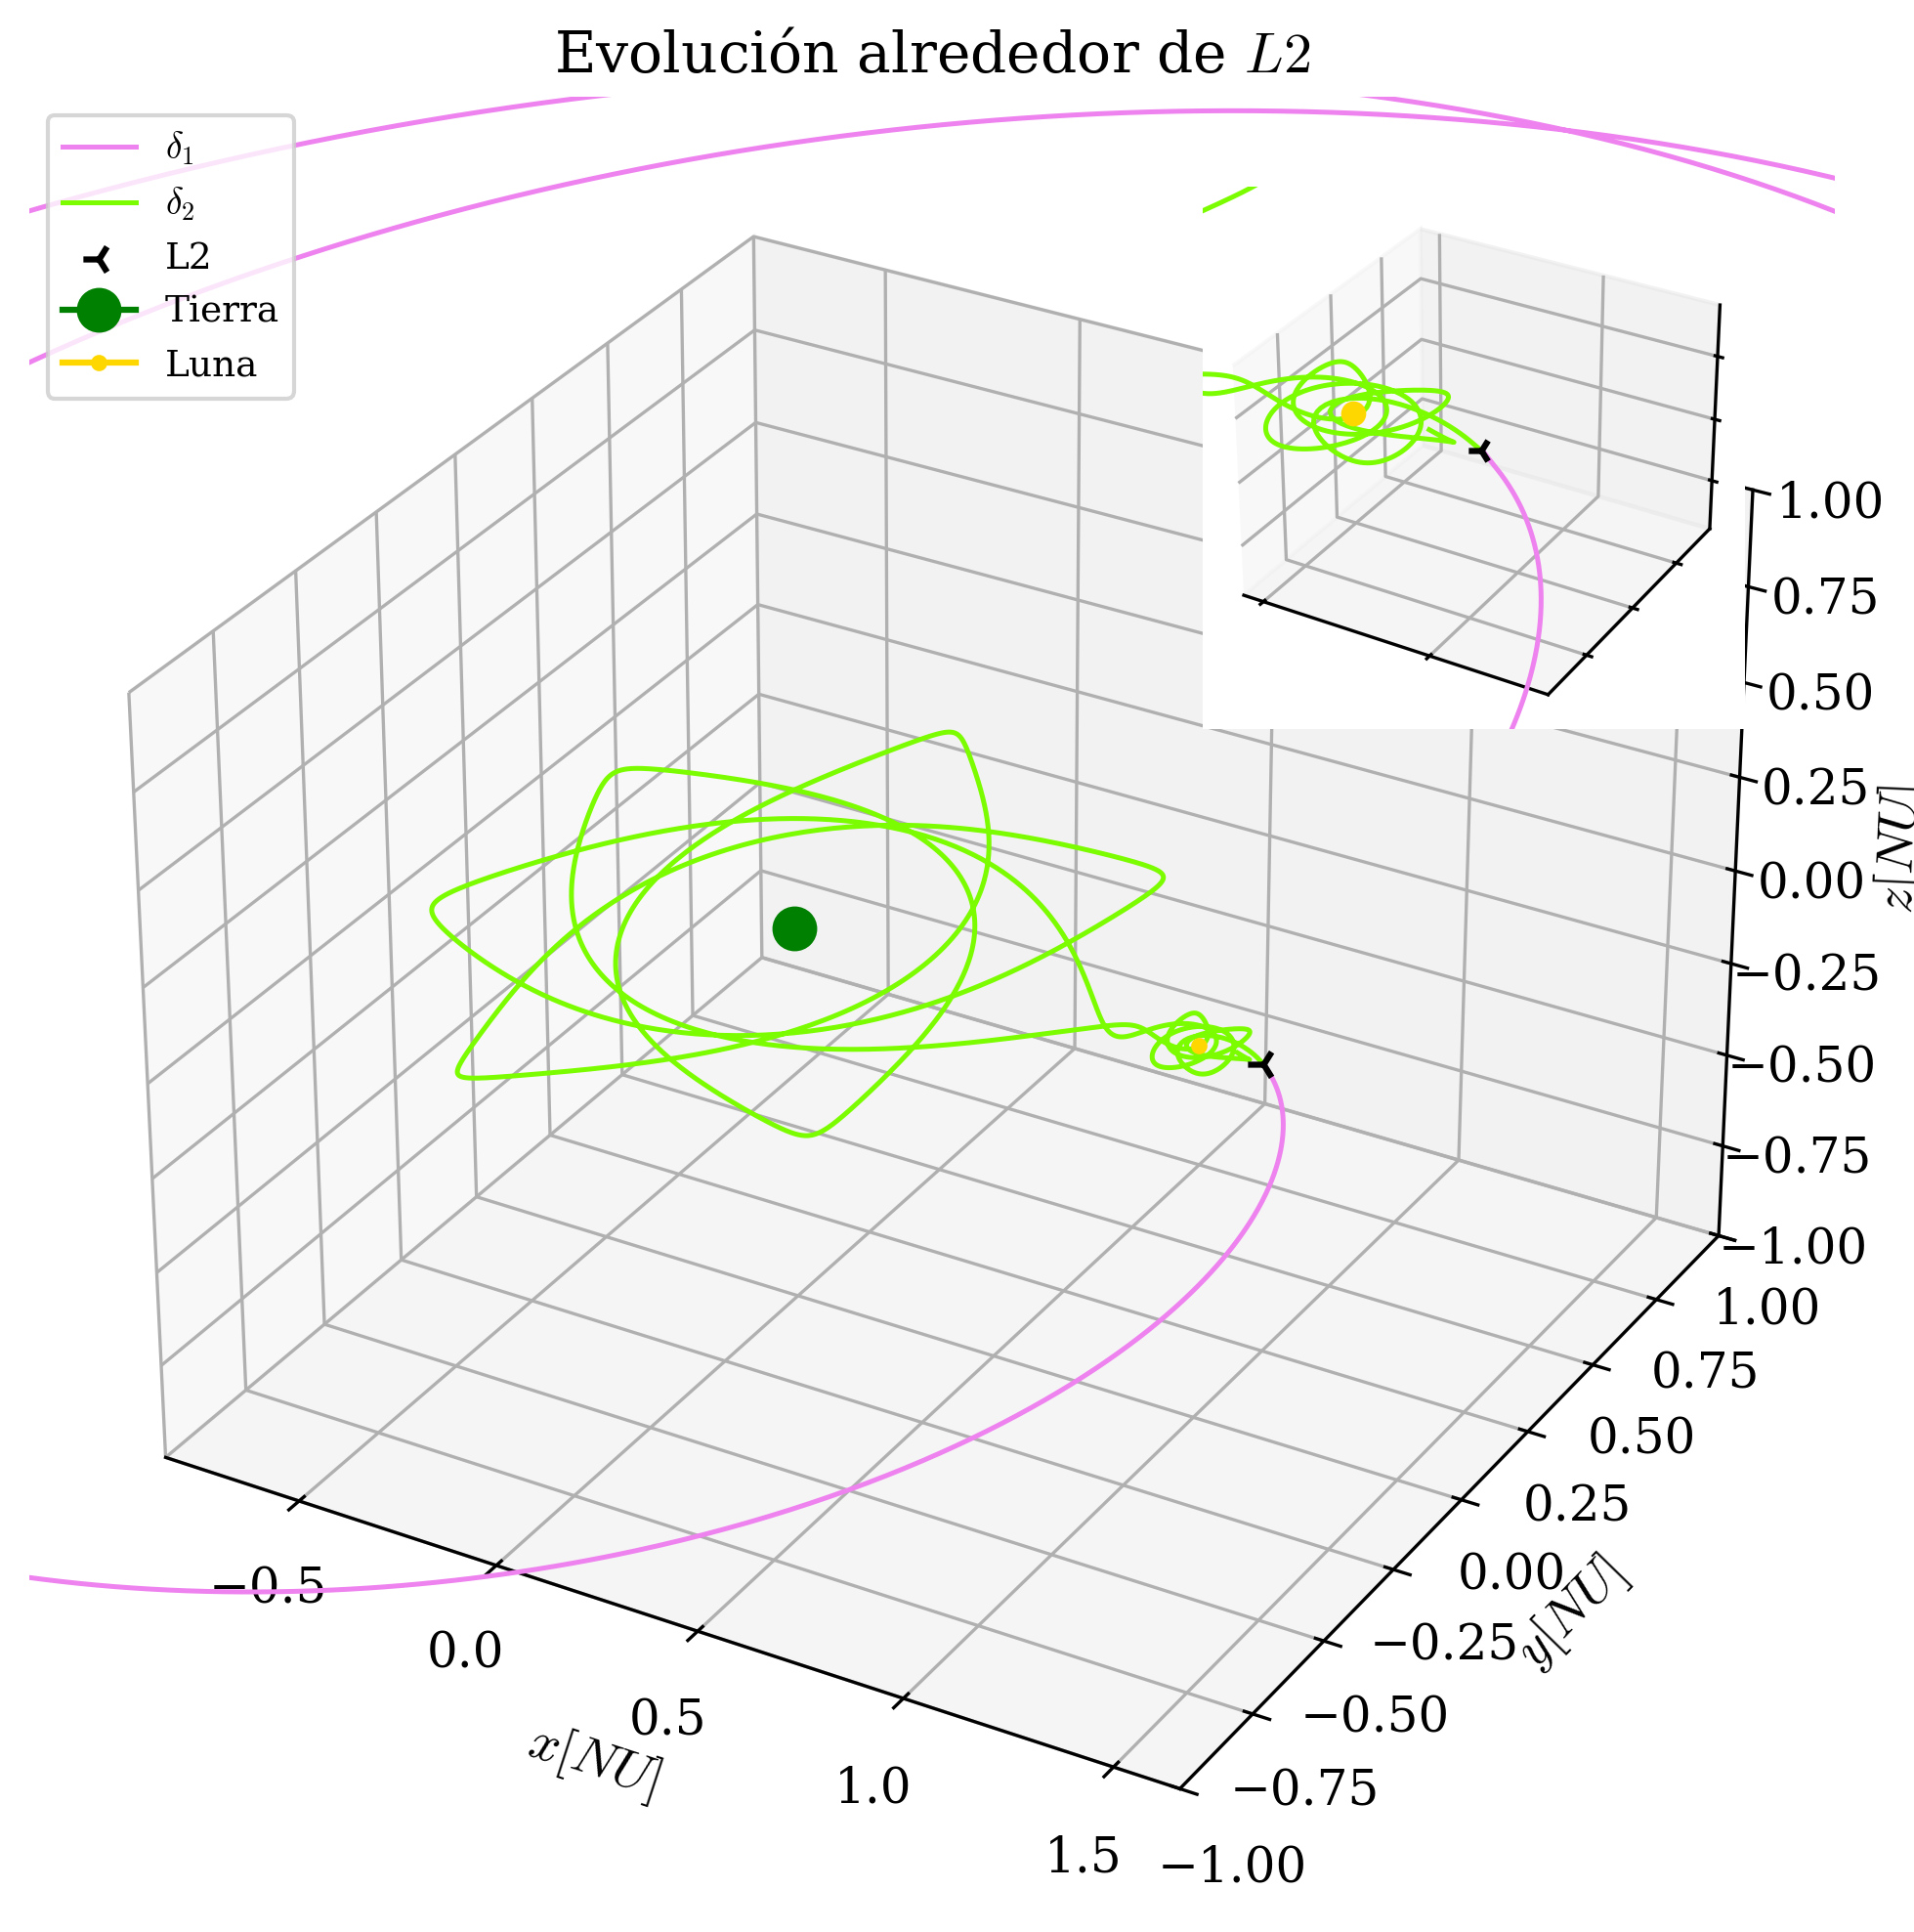
\includegraphics[width=\textwidth]{figures_tex/orbit_lagrange_L2.png}}
    \end{minipage}
    \begin{minipage}{0.48\textwidth}
        \href{https://www.youtube.com/watch?v=1oSx0j2YHP0}{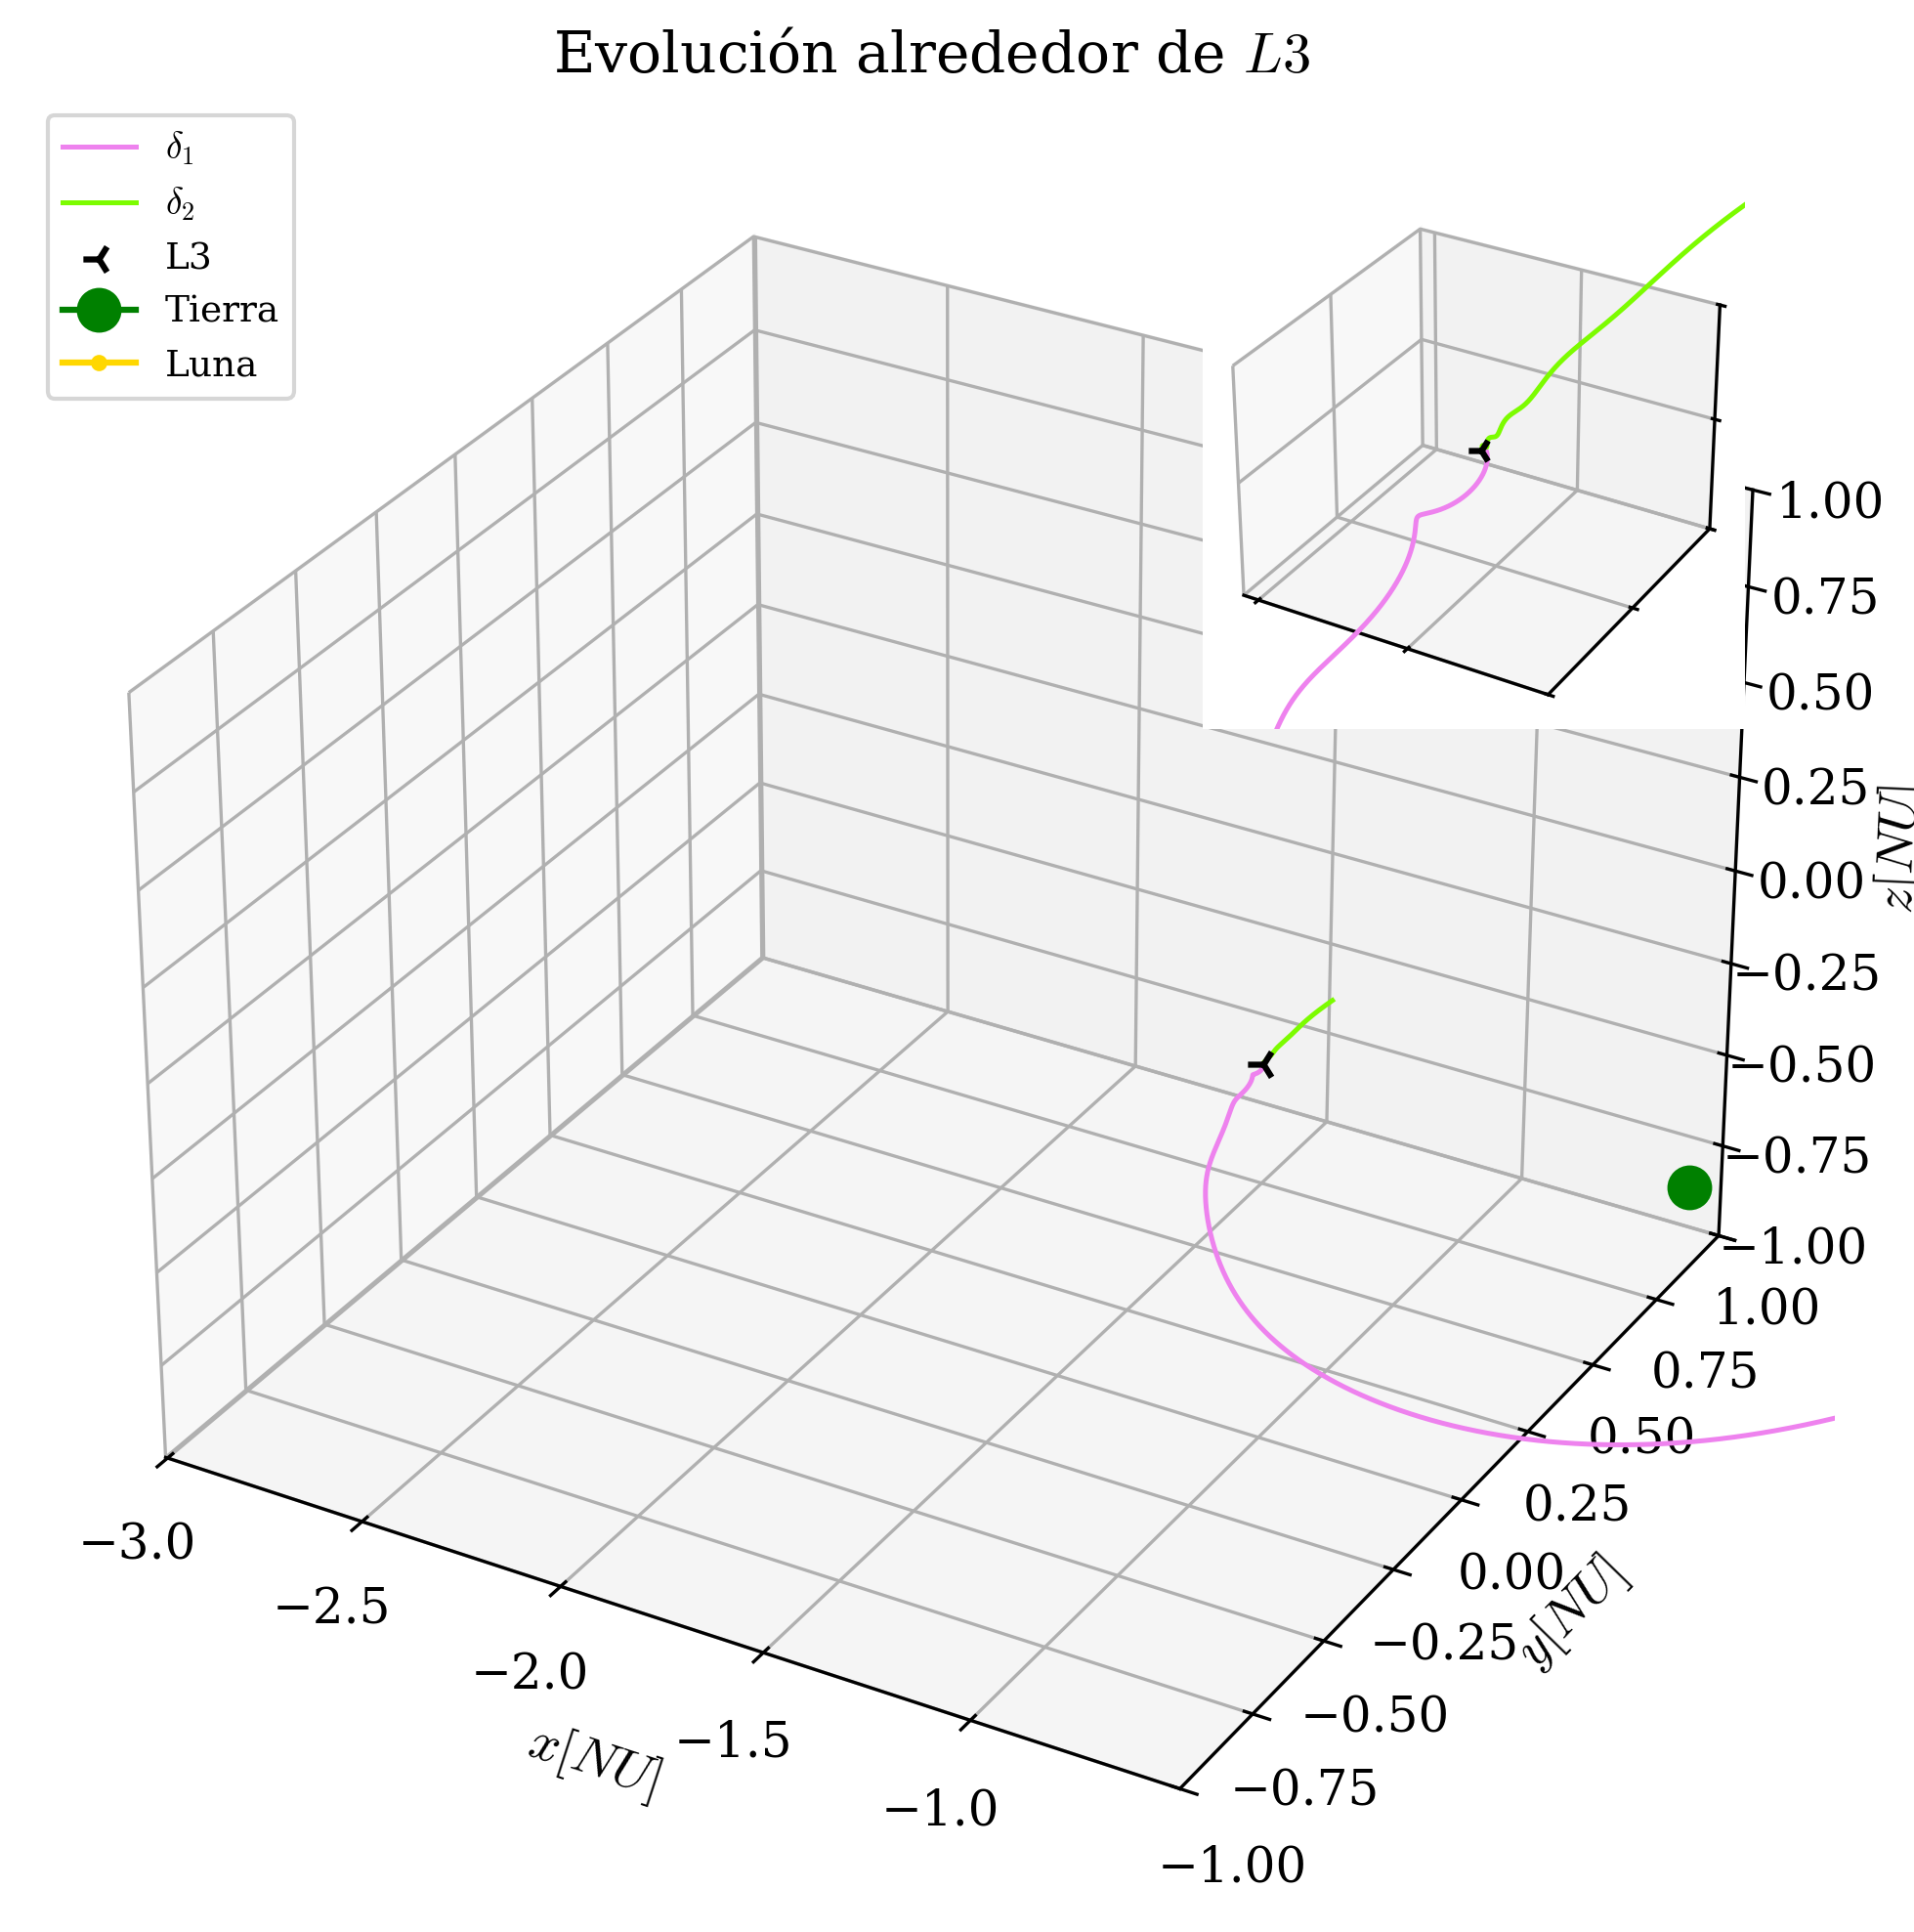
\includegraphics[width=\textwidth]{figures_tex/orbit_lagrange_L3.png}}
    \end{minipage}
    \begin{minipage}{0.48\textwidth}
        \href{https://youtube.com/watch/4zm1RVNYcHc?feature=share}{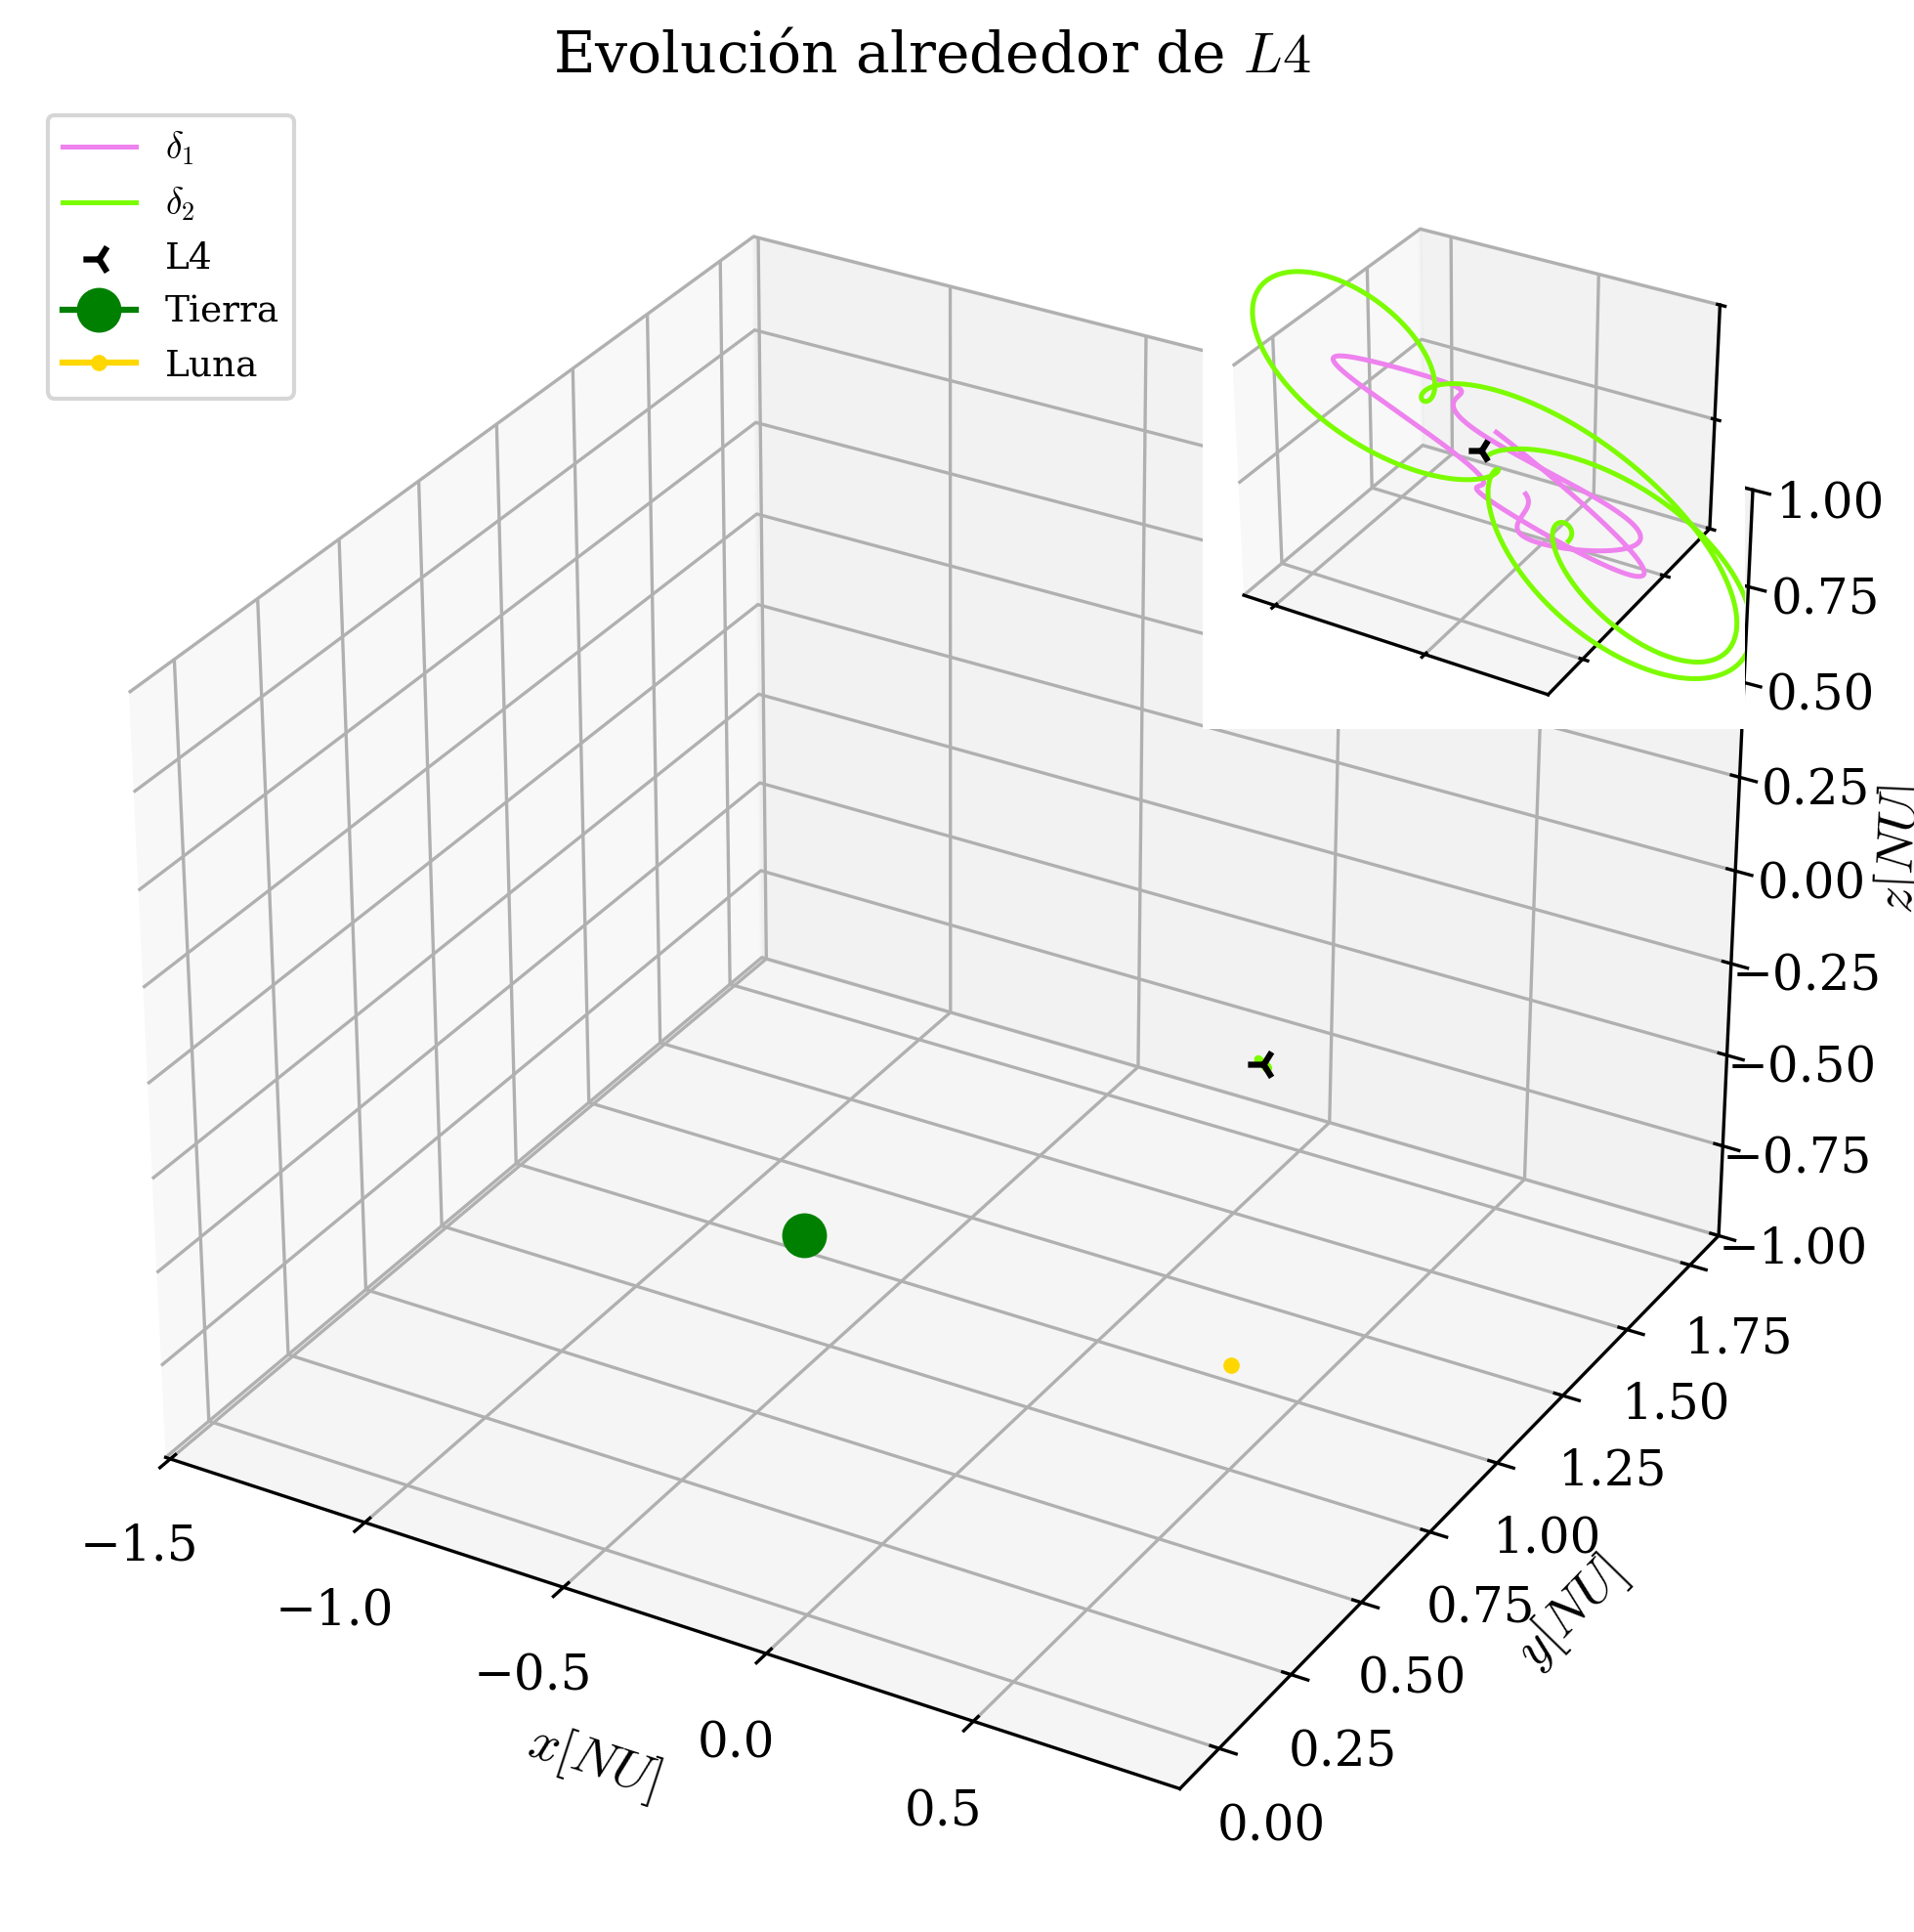
\includegraphics[width=\textwidth]{figures_tex/orbit_lagrange_L4.png}}
    \end{minipage}
    \caption{Evolución de trayectorias perturbadas en la vecindad de $L_1$ (arriba izq.), $L_2$ (arriba der.), $L_3$ (abajo izq.) y $L_4$ (abajo der.). Los recuadros muestran ampliaciones del comportamiento local.}
    \label{fig:lagrange_orbits}
\end{figure}

En los puntos colineales ($L_1, L_2, L_3$), las variaciones iniciales $\delta_i$ provocan una divergencia rápida, llevando a las masas de prueba a trayectorias de escape erráticas. En $L_4$, la masa de prueba permanece confinada, trazando órbitas complejas acotadas.
